\documentclass[%
    %draft,
    %submission,
    %compressed,
    final,
    %
    %technote,
    %internal,
    %submitted,
    %inpress,
    reprint,
    %
    %titlepage,
    notitlepage,
    %anonymous,
    narroweqnarray,
    inline,
    twoside,
    invited
    ]{ieee}

\usepackage[utf8]{inputenc}
\usepackage[spanish]{babel}
\usepackage{graphicx}
\usepackage{verbatim}
\usepackage{moreverb}
\usepackage{amsmath}
\usepackage{amsfonts}
\usepackage{amssymb}
\usepackage{fancybox}
\usepackage{float}
\usepackage{fancyvrb}
\usepackage{subfigure}

\newcommand{\latexiie}{\LaTeX2{\Large$_\varepsilon$}}

%\usepackage{ieeetsp}    % if you want the "trans. sig. pro." style
%\usepackage{ieeetc}    % if you want the "trans. comp." style
%\usepackage{ieeeimtc}    % if you want the IMTC conference style

% Use the `endfloat' package to move figures and tables to the end
% of the paper. Useful for `submission' mode.
%\usepackage {endfloat}

% Use the `times' package to use Helvetica and Times-Roman fonts
% instead of the standard Computer Modern fonts. Useful for the 
% IEEE Computer Society transactions.
%\usepackage{times}
% (Note: If you have the commercial package `mathtime,' (from 
% y&y (http://www.yandy.com), it is much better, but the `times' 
% package works too). So, if you have it...
%\usepackage {mathtime}

% for any plug-in code... insert it here. For example, the CDC style...
%\usepackage{ieeecdc}

\begin{document}

%----------------------------------------------------------------------
% Title Information, Abstract and Keywords
%----------------------------------------------------------------------
\title[Redes Neuronales]{%
       Redes Neuronales}

% format author this way for journal articles.
% MAKE SURE THERE ARE NO SPACES BEFORE A \member OR \authorinfo
% COMMAND (this also means `don't break the line before these
% commands).
\author[Castiglione, Karpovsky, Sturla]{Gonzalo V. Castiglione, Alan E. Karpovsky, Martín Sturla\\\textit{Estudiantes 
       Instituto Tecnológico de Buenos Aires (ITBA)}\\
\textbf{12 de Abril de 2012}
}



\journal{Cátedra\ \ Sist.\ de\ Inteligencia\ Artificial,\ ITBA\ }
\titletext{-\ 12, ABRIL\ 2012}
\ieeecopyright{\copyright\ 2012 ITBA}
\lognumber{}
\pubitemident{}
\loginfo{12 de Abril, 2012.}
\firstpage{1}

\confplacedate{Buenos Aires, Argentina, 12 de Abril, 2012}

\maketitle               

\begin{abstract} 
El presente informe busca analizar  redes neuronales 
con aprendizaje supervisado que resuelvan el problema del \textit{AND} y \textit{OR} lógico para $N$ bits 
con $2 \le N \le 5$ a través del uso de tres variantes de funciones de transferencia.

\end{abstract}

\begin{keywords}
perceptrón, función de transferencia, red neuronal, aprendizaje supervisado, conjunto de entrenamiento, conjunto de testeo
\end{keywords}

%----------------------------------------------------------------------
% SECTION I: Introduccion%----------------------------------------------------------------------
\section{Introducción}

\PARstart Las redes neuronales son un paradigma de aprendizaje y procesamiento automático inspirado 
en la forma en que funciona el sistema nervioso de los animales. Se trata de un sistema de interconexión de 
neuronas en una red que colabora para producir un estímulo de salida. Cabe destacarse que las redes neuronales no 
dejan de ser un modelo y es debido a esto que no tienen en cuenta muchas de las funciones y cualidades del cerebro humano.

%----------------------------------------------------------------------
% SECTION II: Marco Teórico
%----------------------------------------------------------------------

\section{Desarrollo}

\subsection{Modelado del problema}

\par Se representó la red neuronal como una \textbf{matriz de pesos}. Cada neurona es una columna de pesos, cada capa de 
neuronas es una matriz de pesos, la red neuronal, por consiguiente, es un vector de matrices (en particular un 
perceptrón simple es solo una matriz). Lo interesante es que hallar 
el valor de la red neuronal con un cierto input se reduce a multiplicar el vector entrada por cada una de estas matrices. Cabe destacar 
que al vector de entrada se le agrega siempre un $-1$ como último valor para el sesgo.
A su vez esta implementación facilita el manejo de errores.\\

\par Para las unidades escalón el error está definido como la \textbf{Distancia Hamming Levenshtein}, 
para los otros tipos de unidades se decidió utilizar el \textbf{error cuadrático medio}.

\subsection{Features}

\par Se implementaron tres tipos de funciones para modificar la variable $\eta$ \textit{(learn rate)}: 
La primera de ellas es a valor \textbf{constante}, , la segunda es \textbf{\textit{annealed}} que reduce $\eta$ exponencialmente y por último se 
tiene un \textit{learning rate} \textbf{adaptative} que modifica $\eta$ en función de los últimos errores obtenidos. El crecimiento es aritmético, con cota 
en $\eta =0.5$, la reducción exponencial.

\subsection{Ejecución}

\par La implementación considera la llamada a una única función \textit{main} a la que se le pasan los siguientes parámetros de configuración: operación lógica (AND / OR), cantidad de bits (entre 2 y 5), cantidad de épocas, eta ($\eta$), tipo de aprendizaje \textit{constant, annealed, dynamic} en ese órden.
Por ejemplo la siguiente llamada:

\begin{verbatim}
main('AND', N, 500, 'SIGMOID', 0.02, 'COSNTANT')
\end{verbatim}

Le pasará al perceptrón simple el problema del AND lógico de N bits, con la función de transferencia sigmoidea, $\eta=0.02$, tipo de aprendizaje constante y correrá por 500 épocas.\\
Cabe destacar que el conjunto de entrenamiento está compuesto por todos los casos posibles (al igual que el de testeo) y en cada época se altera el orden de 
dicho conjunto.

\section{Resultados}

\par A modo de ejemplo, en la sección \textit{\textbf{Anexo A}} se puede observar una tabla comparativa entre los distintos tipos de funciones 
de transferencia para un $\eta$ pequeño, con tipo de aprendizaje constante. Se decidió duplicar la cantidad de épocas tomadas inicialmente a
 medida que se incrementaba la cantidad de \textit{inputs}.

\par Como se puede apreciar en las tablas, las unidades escalón probaron ser las más rápidas en reducir el error.

\section{Conclusión}

\PARstart Luego de realizar numerosas pruebas variando los parámetros de configuración de la red neuronal, 
podemos concluír que hemos tenido mejores resultados utilizando $\beta=1$ y utilizando valores más altos de $\eta$. 
Esto puede deberse posiblemente a la naturaleza planar del problema.

\par Al oservar los gráficos de error obtenidos al realizar pruebas con funciones sigmoideas y lineales, 
notamos que el error tiende a cero, pero lo hace más rápido utilizando el $eta$ en modo \textit{adaptative}
. Este fenómeno puede ser observado en el \textit{\textbf{Anexo B}} donde se compara 
el error obtenido con un $\eta$ constante versus un $\eta$ adaptativo.

%\begin{thebibliography}{1}

%\bibitem{lamport1}
%Fierens, P. (2011),
%\newblock {\em Cuadrados mínimos: repaso},
%\newblock Buenos Aires: Instituto Tecnológico de Buenos Aires.

%\bibitem{lamport1}
%Abdi, H.,
%\newblock {\em  Least-squares: {Encyclopedia for research methods for the social sciences}},
%\newblock Thousand Oaks (CA): Sage. pp, 2003.

%\bibitem{lamport1}
%Farebrother, R.W. (1988),
%\newblock {\em Linear Least Squares Computations, STATISTICS: Textbooks and Monographs}, %\newblock New York: Marcel Dekker.

%\bibitem{lamport1}
%Lipson, M.; Lipschutz, S. (2001),
%\newblock {\em Schaum's outline of theory and problems of linear algebra}, 
%newblock New York: McGraw-Hill, pp. 69–80.


%\end{thebibliography}

%----------------------------------------------------------------------


\clearpage
\onecolumn
\section*{Anexo A: Tablas}
 
\begin{center}
\textbf{\emph{AND}}
\end{center}

\begin{table}[H]
\begin{center}
\begin{tabular}{|c|c|c|c|c|}
\hline
Bits &  Eta & Función de &  Épocas & Error de\\
 & $\eta$ & activación &  & aprendizaje\\

\hline
\hline

2 & 0.02 & Escalón & 50 & 0\\
\hline
2 & 0.02 & Lineal & 50 & 0.287\\
\hline
2 & 0.02 & Sigmóidea & 50 & 0.571\\
\hline
\hline
3 & 0.02 & Escalón & 100 & 0\\
\hline
3 & 0.02 & Lineal & 100 & 0.256\\
\hline
3 & 0.02 & Sigmóidea & 100 & 0.581\\
\hline
\hline
4 & 0.02 & Escalón & 200 & 0\\
\hline
4 & 0.02 & Lineal & 200 & 0.181\\
\hline
4 & 0.02 & Sigmóidea & 200 & 0.523\\
\hline
\hline
5 & 0.02 & Escalón & 400 & 0\\
\hline
5 & 0.02 & Lineal & 400 & 0.089\\
\hline
5 & 0.02 & Sigmóidea & 400 & 0.421\\
\hline

\end{tabular}
\end{center}
\caption{Comparación de errores de la salida de la red para AND lógico con tipo de aprendizaje constante}\label{tablaIDFS}
\end{table}

\begin{center}
\textbf{\emph{OR}}
\end{center}

\begin{table}[H]
\begin{center}
\begin{tabular}{|c|c|c|c|c|}
\hline
Bits &  Eta & Función de &  Épocas & Error de\\
 & $\eta$ & activación &  & aprendizaje\\

\hline
\hline

2 & 0.02 & Escalón & 50 & 0\\
\hline
2 & 0.02 & Lineal & 50 & 0.310\\
\hline
2 & 0.02 & Sigmóidea & 50 & 0.545\\
\hline
\hline
3 & 0.02 & Escalón & 100 & 0\\
\hline
3 & 0.02 & Lineal & 100 & 0.258\\
\hline
3 & 0.02 & Sigmóidea & 100 & 0.568\\
\hline
\hline
4 & 0.02 & Escalón & 200 & 0\\
\hline
4 & 0.02 & Lineal & 200 & 0.181\\
\hline
4 & 0.02 & Sigmóidea & 200 & 0.520\\
\hline
\hline
5 & 0.02 & Escalón & 400 & 0\\
\hline
5 & 0.02 & Lineal & 400 & 0.089\\
\hline
5 & 0.02 & Sigmóidea & 400 & 0.425\\
\hline

\end{tabular}
\end{center}
\caption{Comparación de errores de la salida de la red para OR lógico con tipo de aprendizaje constante}\label{tablaIDFS}
\end{table}

\clearpage

\section*{Anexo B: Gráficos}


\begin{figure}[H]
\begin{center}
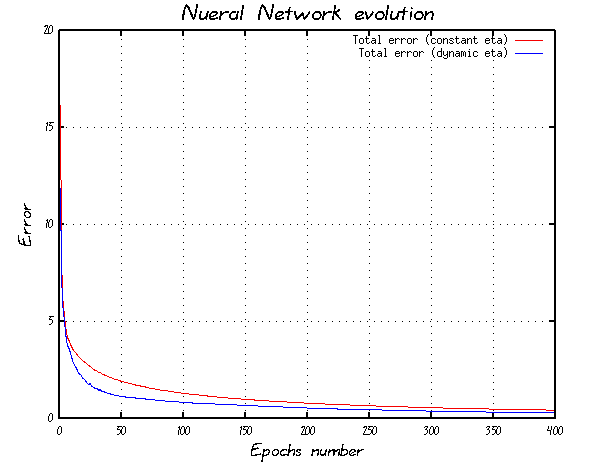
\includegraphics[scale=0.85]{./images/g1.png}
\label{modelado}
\end{center}
\end{figure}

\begin{center}
\par Figura 1: Curva de error con eta constante vs. eta dinámico
\end{center}



%\VerbatimInput{./code/calculoAb.m}




\end{document}